\documentclass[12pt, openany, oneside]{book}

\usepackage{listings}
\usepackage[dvipsnames]{xcolor}
\usepackage{ctex}
\usepackage{fontspec}
\usepackage{setspace}
\usepackage{tikz}
\usepackage{anyfontsize}
\usepackage{sectsty}
\usepackage{titlesec}
\usepackage{float}
\usepackage[hidelinks]{hyperref}
\usepackage[a4paper]{geometry}
\usepackage{url}
\usepackage{amssymb}
\usepackage{fontawesome5}
\usepackage[most]{tcolorbox}
\usepackage{stackengine}
\usepackage{multirow}
\usepackage{textcomp}
\usepackage[T1]{fontenc}
% \usepackage{minted}

\lstset{upquote=true}

\usetikzlibrary{calc,trees,positioning,arrows,fit,shapes,calc}

\def\rlwd{.5pt} \def\rlht{2.2ex} \def\rldp{.5ex}
\def\mydiv#1{~%
  \rule[-\rldp]{\rlwd}{\rlht}%
  \setbox0=\hbox{~#1}%
  \stackunder[\dimexpr\rldp-\rlwd]{~#1}{\rule{\wd0}{\rlwd}}%
}

\definecolor{mycolor}{RGB}{0,128,128}
\newtcbox{\mybox} {
    on line,
    colback=mycolor,
    fontupper=\bfseries\color{white},
    boxrule=0pt,
    arc=5pt, 
    boxsep=0pt, 
    left=2pt, 
    right=2pt, 
    top=5pt, 
    bottom=5pt
}

\setstretch{1.5}
\setlength{\parindent}{0cm}

\geometry{a4paper,top=2.5cm,bottom=2.5cm}

\titleformat{\chapter}{\Huge\Huge\bfseries}{\chaptertitlename\ \thechapter{\ }}{0pt}{\Huge}{}
\titlespacing{\chapter}{0pt}{0pt}{12pt}

\definecolor{lightgray}{rgb}{0.95, 0.95, 0.95}
\definecolor{darkgray}{rgb}{0.4, 0.4, 0.4}
\definecolor{editorGray}{rgb}{0.95, 0.95, 0.95}
\definecolor{editorOcher}{rgb}{1, 0.5, 0} % #FF7F00 -> rgb(239, 169, 0)
\definecolor{editorGreen}{rgb}{0, 0.5, 0} % #007C00 -> rgb(0, 124, 0)
\definecolor{orange}{rgb}{1,0.45,0.13}		
\definecolor{olive}{rgb}{0.17,0.59,0.20}
\definecolor{brown}{rgb}{0.69,0.31,0.31}
\definecolor{purple}{rgb}{0.38,0.18,0.81}
\definecolor{lightblue}{rgb}{0.1,0.57,0.7}
\definecolor{lightred}{rgb}{1,0.4,0.5}

\lstdefinelanguage{HTML5}{
  language=html,
  sensitive=true,	
  alsoletter={<>=-},	
  morecomment=[s]{<!--}{-->},
  tag=[s],
  otherkeywords={
  % Standard tags
	<html, <meta, </html>, <link,
	</body>, <body>,
	<div>, </div>, 
	<p>, </p>, <p,
	</script>, <script>,
	<span>, </span>,
	<h1>, </h1>, <h1,
	<h2>, </h2>, <h2,
	<h3>, </h3>, <h3,
	<h4>, </h4>, <h4,
	<h5>, </h5>, <h5,
	<h6>, </h6>, <h6,
	<head>, </head>,
	<title>, </title>,
	<style>, </style>, <style,
	<ol>, </ol>, <ol,
	<ul>, </ul>, <ul,
	<li>, </li>,
	<br/>, <br />, <br>,
	<hr/>, <hr />, <hr>, 
	<img/>, <img />, <img>, <img,
	&nbsp;,
	<a>, </a>, <a,
	<div>, </div>, <div,
	<table>, </table>, <table,
	<input,
	<caption>, </caption>,
	<tr>, </tr>,
	<th>, </th>,
	<td>, </td>,
	<form>, </form>, <form,
	<textarea>, </textarea>, <textarea,
	<label>, <label, </label>,
	<select>, </select>,
	<option>, </option>, <option,
  % More tags...
  <canvas, /canvas>, <svg, <rect, <animateTransform, </rect>, </svg>, <video, <source, <iframe, </iframe>, </video>, <image, </image>, <header, </header, <article, </article
  },
  ndkeywords={
  % General
  =,
  % HTML attributes
  lang=, charset=, src=, id=, width=, height=, style=, type=, rel=, href=, alt=, title=, border=,
  method=, action=, name=, value=, placeholder=, for=, rows=, cols=, checked=, selected=,
  % SVG attributes
  fill=, attributeName=, begin=, dur=, from=, to=, poster=, controls=, x=, y=, repeatCount=, xlink:href=,
  % properties
  color:, margin:, padding:, background-image:, border:, top:, left:, position:, width:, height:, margin-top:, margin-bottom:, font-size:, line-height:, text-align:,
  background-color:, border-radius:, cursor:, float:, list-style:,
  font-family:, font-weight:, font-style:,
	% CSS3 properties
  transform:, -moz-transform:, -webkit-transform:,
  animation:, -webkit-animation:,
  transition:,  transition-duration:, transition-property:, transition-timing-function:,
  }
}

\lstdefinelanguage{CSS}{
  keywords={background-image:,margin,padding,font,weight,display,position,top,left,right,bottom,list,style,border,size,white,space,min,width, transition:, transform:, transition-property, transition-duration, transition-timing-function},	
  sensitive=true,
  morecomment=[l]{//},
  morecomment=[s]{/*}{*/},
  morestring=[b]',
  morestring=[b]",
  alsoletter={:},
  alsodigit={-},
}

\lstdefinelanguage{JavaScript}{
  morekeywords={typeof, new, true, false, catch, function, return, null, catch, switch, var, if, in, while, do, else, case, break},
  morecomment=[s]{/*}{*/},
  morecomment=[l]//,
  morestring=[b]",
  morestring=[b]'
}

\lstdefinestyle{htmlcssjs} {
    % General design
    %  backgroundcolor=\color{editorGray},
    basicstyle=\linespread{1.3} \fontspec{Consolas},    %  the size of the fonts that are used for the code
    basewidth=0.5em,
    numbers=left,            % where to put the line-numbers
    numberstyle=\color{black},  % the style that is used for the line-numbers
    numbersep=10pt,                  % how far the line-numbers are from the code
    backgroundcolor=\color{white},
    showspaces=false,
    showstringspaces=false,
    showtabs=false,
    frame=single,                   % adds a frame around the code
    rulecolor=\color{black},        % if not set, the frame-color may be changed on line-breaks within not-black text (e.g. commens (green here))
    tabsize=4,                      % sets default tabsize to 2 spaces
    captionpos=t,                   % sets the caption-position to bottom
    breaklines=false,                % sets automatic line breaking
    breakatwhitespace=true,        % sets if automatic breaks should only happen at whitespace
    % line-numbers
    xleftmargin={0.75cm},
    stepnumber=1,
    firstnumber=1,
    numberfirstline=true,	
    % Code design
    identifierstyle=\color{black},
    keywordstyle=\color{blue}\bfseries,
    ndkeywordstyle=\color{editorGreen}\bfseries,
    stringstyle=\color{editorOcher}\ttfamily,
    commentstyle=\color{brown}\ttfamily,
    % Code
    language=HTML5,
    alsolanguage=JavaScript,
    alsodigit={.:;},	
    extendedchars=true,
    breaklines=true,
    % German umlauts
    literate=%
    {Ö}{{\"O}}1
    {Ä}{{\"A}}1
    {Ü}{{\"U}}1
    {ß}{{\ss}}1
    {ü}{{\"u}}1
    {ä}{{\"a}}1
    {ö}{{\"o}}1
}

\begin{document}

\pagestyle{plain}

\begin{tikzpicture}[overlay,remember picture]
	% Background color
	\fill[
		black!2]
	(current page.south west) rectangle (current page.north east);

	% Rectangles
	\shade[
		left color=Dandelion,
		right color=Dandelion!40,
		transform canvas ={rotate around ={45:($(current page.north west)+(0,-6)$)}}]
	($(current page.north west)+(0,-6)$) rectangle ++(9,1.5);

	\shade[
		left color=lightgray,
		right color=lightgray!50,
		rounded corners=0.75cm,
		transform canvas ={rotate around ={45:($(current page.north west)+(.5,-10)$)}}]
	($(current page.north west)+(0.5,-10)$) rectangle ++(15,1.5);

	\shade[
		left color=lightgray,
		rounded corners=0.3cm,
		transform canvas ={rotate around ={45:($(current page.north west)+(.5,-10)$)}}] ($(current page.north west)+(1.5,-9.55)$) rectangle ++(7,.6);

	\shade[
		left color=orange!80,
		right color=orange!60,
		rounded corners=0.4cm,
		transform canvas ={rotate around ={45:($(current page.north)+(-1.5,-3)$)}}]
	($(current page.north)+(-1.5,-3)$) rectangle ++(9,0.8);

	\shade[
		left color=red!80,
		right color=red!80,
		rounded corners=0.9cm,
		transform canvas ={rotate around ={45:($(current page.north)+(-3,-8)$)}}] ($(current page.north)+(-3,-8)$) rectangle ++(15,1.8);

	\shade[
		left color=orange,
		right color=Dandelion,
		rounded corners=0.9cm,
		transform canvas ={rotate around ={45:($(current page.north west)+(4,-15.5)$)}}]
	($(current page.north west)+(4,-15.5)$) rectangle ++(30,1.8);

	\shade[
		left color=RoyalBlue,
		right color=Emerald,
		rounded corners=0.75cm,
		transform canvas ={rotate around ={45:($(current page.north west)+(13,-10)$)}}]
	($(current page.north west)+(13,-10)$) rectangle ++(15,1.5);

	\shade[
		left color=lightgray,
		rounded corners=0.3cm,
		transform canvas ={rotate around ={45:($(current page.north west)+(18,-8)$)}}]
	($(current page.north west)+(18,-8)$) rectangle ++(15,0.6);

	\shade[
		left color=lightgray,
		rounded corners=0.4cm,
		transform canvas ={rotate around ={45:($(current page.north west)+(19,-5.65)$)}}]
	($(current page.north west)+(19,-5.65)$) rectangle ++(15,0.8);

	\shade[
		left color=OrangeRed,
		right color=red!80,
		rounded corners=0.6cm,
		transform canvas ={rotate around ={45:($(current page.north west)+(20,-9)$)}}]
	($(current page.north west)+(20,-9)$) rectangle ++(14,1.2);

	% Year
	% \draw[ultra thick,gray]
	% ($(current page.center)+(5,2)$) -- ++(0,-3cm)
	node[
			midway,
			left=0.25cm,
			text width=5cm,
			align=right,
			black!75
		]
		{
			% {\fontsize{25}{30} \selectfont \bf ANNUAL \\[10pt] REPORT}
		}
	node[
			midway,
			right=0.25cm,
			text width=6cm,
			align=left,
			orange]
		{
			% {\fontsize{72}{86.4} \selectfont 2020}
		};

	% Title
	\node[align=center] at ($(current page.center)+(0,-6)$)
	{
	{\fontsize{50}{50} \selectfont {{HTML/CSS/JavsScript}}} \\[2cm]
	{\fontsize{20}{19.2} \selectfont \textcolor{orange}{\bf 极夜酱}} \\[4pt]
	};
\end{tikzpicture}

\newpage

\setcounter{tocdepth}{1}
\tableofcontents
\thispagestyle{empty}

\newpage

\setcounter{page}{1}

\part{HTML}

\newpage

\chapter{HTML简介}

\section{前后端}

\subsection{前端工程师(Front-End Engineer)}

前端工程师互联网时代软件产品研发中不可缺少的一种专业研发角色。前端是一个相对比较新的行业,大约从2005年开始,正式的前端工程师角色被行业所认可。到了2010年,互联网开始全面进入移动时代,前端工程师的地位也越来越重要。 \\

现在一些后端开发工作也可以由前端工程师来完成。最初所有的开发工作都是由后端工程师完成的,但是随着业务越来越繁杂、工作量过大,后端工程师们不堪重负,于是将可视化和部分交互功能的开发剥离出来,形成了前端开发。 \\

前端工程师主要负责的工作就是使用HTML、CSS、JavaScript等专业技能和工具将产品UI设计稿实现成网站产品。涵盖用户PC端和移动端网页,处理视觉和交互问题。 \\

广义上讲,所有用户终端产品,只要是与视觉和交互有关的部分都是前端工程师的专业领域。产品从前期开发到后期的维护、更新、升级都需要前端工程师来完成。

\subsection{后端工程师(Back-End Engineer)}

后端工程师主要负责服务器的数据逻辑和业务逻辑等,主要研究怎么把数据更好地传输给前端工程师。 \\

如果一个人除了完成前端开发和后端开发工作以外,从产品设计到项目开发,再到后期运维都是同一个人,甚至可能还要负责UI、配动画、写文档等,那么就被称为全栈工程师(Full Stack Engineer)。

\subsection{前端应用领域}

前端技术可以被应用在一系列领域中:

\begin{itemize}
	\item 网页网站
	\item APP、微信小程序
	\item 移动端小游戏
	\item 炫酷的特效
	\item 大数据可视化
	\item VR虚拟现实
\end{itemize}

前端工程师需要具备大量必要的技能,其中前端三大基础语言为HTML、CSS、JavaScript,除此之外还需要学习jQuery、网络、es6、webpack4.0、小程序、VUE、React、Node.js、Mongo DB数据库等内容。 \\

\newpage

\section{结构层/表现层/行为层}

\subsection{结构层/表现层/行为层}

\begin{itemize}
	\item 结构层HTML(HyperText Markup Language):一个超文本标记语言,负责描绘出网页内容的架构。

	\item 表示层CSS(Cascading Style Sheets):层叠样式表,负责如何显示结构层的有关内容。

	\item 行为层JavaScript:目前在Web上使用的最主要的客户端脚本语言,是Web脚本语言的一个标准,可以对结构层和表现层的内容随意进行更改。
\end{itemize}

\subsection{代码注释}

在HTML、CSS、JavaScript中代码的注释是不一样的。

\begin{lstlisting}[style=htmlcssjs, title=HTML注释,keywordstyle=\color{brown},]
<!-- 注释内容 -->
\end{lstlisting}

\begin{lstlisting}[style=htmlcssjs, title=CSS注释]
/* 注释内容 */
\end{lstlisting}

\begin{lstlisting}[style=htmlcssjs, title=JavaScript注释]
// 注释内容
/* 注释内容 */
\end{lstlisting}

\newpage

\section{Hello World!}

\subsection{Hello World!}

问候一下世界,制作人生中的第一个HTML网页吧。

\begin{lstlisting}[style=htmlcssjs, title=Hello World!]
<!DOCTYPE html>
<html lang="en">
<head>
    <meta charset="UTF-8">
    <title>Hello World!</title>
</head>
<body>
    Hello World!
</body>
</html>
\end{lstlisting}

\subsection{HTML和CSS的关系}

先来看一下单纯的HTML标签长什么样:

\begin{figure}[H]
	\centering
	
\includegraphics[]{img/C1/1-3/1.png}
\end{figure}

再来看一下经过CSS修饰过后的HTML标签:

\begin{lstlisting}[style=htmlcssjs, title=Hello World!]
p {
    color: red;
    border: 1px solid red;
    width: 140px;
    height: 40px;
}
\end{lstlisting}

\begin{figure}[H]
	\centering
	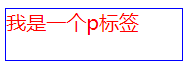
\includegraphics[]{img/C1/1-3/2.png}
\end{figure}

CSS是用来修饰HTML样式的。虽然HTML本身是有一些默认样式,但如果想改变HTML标签的样式,就需要借助CSS。 \\

HTML + CSS构成了网页的基本页面结构和样式。

\begin{lstlisting}[style=htmlcssjs, title=添加样式]
<!DOCTYPE html>
<html lang="en">
<head>
    <meta charset="UTF-8">
    <title>添加样式</title>
    <style type="text/css">
        p {
            font-size: 12px;
            color: #930;
            text-align: center;
        }
    </style>
</head>
<body>
    <p>Hello World!</p>
</body>
</html>
\end{lstlisting}

\newpage

\section{标签}

\subsection{标签}

HTML中标签的语法有以下几点:

\begin{enumerate}
	\item 标签(tag)是由英文尖括号【<】和【>】括起来的,如\lstinline|<html>|就是一个标签。

	\item HTML中的标签一般都是成对出现的,分开始标签和结束标签。结束标签比开始标签多了一个【/】。
	      \begin{lstlisting}[style=htmlcssjs]
<p></p>
<div></div>
<span></span>
    \end{lstlisting}

	\item 标签与标签之间是可以嵌套的,但先后顺序必须保持一致。如,\lstinline|<div>|里嵌套\lstinline|<p>|,那么\lstinline|</p>|必须放在\lstinline|</div>|的前面。
	      \begin{lstlisting}[style=htmlcssjs]
<div><p>Hello World!</p></div>
    \end{lstlisting}

	\item HTML标签不区分大小写,如\lstinline|<h1>|和\lstinline|<H1>|是一样的,但建议小写,因为大部分程序员都已小写为准。
\end{enumerate}

\newpage

\section{HTML文档结构}

\subsection{HTML文档结构}

\begin{lstlisting}[style=htmlcssjs, title=HTML文档结构]
<!DOCTYPE html>
<html lang="en">
<head>
    <meta charset="UTF-8">
    <title>HTML文档结构</title>
</head>
<body>

</body>
</html>
\end{lstlisting}

\begin{itemize}
    \item \lstinline|<!DOCTYPE html>|:文档类型声明,表示该文件为\lstinline|HTML|文件。\lstinline|<!DOCTYPE>|声明必须是\lstinline|HTML|文档的第一行,位于\lstinline|<html>|之前。
    
    \item \lstinline|<html></html>|:\lstinline|<html>|用来标识HTML文档的开始,\lstinline|</html>|位于HTML文档的最后面,用来标识HTML文档的结束。这两个标签对成对存在,中间的部分是文档的头部和主题。
    
    \item \lstinline|<head></head>|:标签包含有关HTML文档的信息,可以包含一些辅助性标签。如\lstinline|<title></title>|、\lstinline|<link />|、\lstinline|<meta />|、\lstinline|<style></style>|、\lstinline|<script></script>|等,浏览器除了会在标题栏显示\lstinline|<title>|元素的内容外,不会向用户显示\lstinline|head|元素内的其他任何内容。
    
    \item \lstinline|<body></body>|:HTML文档的主体部分,在此标签中可以包含\lstinline|<p>|、\lstinline|<h1>|、\lstinline|<br>|等众多标签。\lstinline|<body>|出现在\lstinline|</head>|之后,且必须在闭标签\lstinline|</html>|之前闭合。
\end{itemize}

\newpage

\section{小哥,做头吗?——head标签}

\subsection{head标签}

文档的头部描述了文档的各种属性和信息,包括文档的标题等,绝大多数文档头部包含的数据都不会真正作为内容显示给读者。 \\

\lstinline|head|标签为双标签\lstinline|<head></head>|,表示头部标签,通常用来嵌套\lstinline|meta|、\lstinline|title|、\lstinline|style|等标签。

\begin{itemize}
    \item \lstinline|<title>|:在\lstinline|<title>|和\lstinline|</title>|标签之间的文字内容是网页的标题信息,它会出现在浏览器的标题栏中。网页的\lstinline|<title>|用于告诉用户和搜索引擎这个网页的主要内容是什么,搜索引擎可以通过网页标题,迅速的判断出网页的主题。每个网页的内容都是不同的,每个网页都应该有一个独一无二的title。
    
    \item \lstinline|<meta charset="UTF-8">|:设置当前文件字符编码。
    
    \item \lstinline|<style>|:设置当前文件样式。
\end{itemize}

\newpage

\section{你就是馋人家的身子!——body标签}

\subsection{body标签}

在网页上要展示出来的页面内容一定要放在\lstinline|<body>|中。

\begin{lstlisting}[style=htmlcssjs, title=body标签]
<!DOCTYPE html>
<html lang="en">
<head>
 <meta charset="UTF-8">
 <title>body标签</title>
</head>
<body>
    <!-- 标题标签 -->
    <h1>HTML简介</h1>
    <!-- 段落标签 -->
    <p>HTML的全称为超文本标记语言,是一种标记语言。</p>
    <!-- 段落标签 -->
    <p>它包括一系列标签.可以将网络上的文档格式统一。</p>
</body>
</html>
\end{lstlisting}
\chapter{语义化标签}

\section{开始我们的第一段对话吧}

\subsection{语义化(Semantic)}

学习HTML标签需要注意标签的用途和标签在浏览器中的默认样式。 \\

语义化,通俗的讲就是明白每个标签的用途,即在什么情况下使用此标签合理。比如,网页上文章的标题可以用标题标签、各个栏目的名称也可以使用标题标签、文章内容的段落就得放在段落标签中。 \\

语义化可以带来一些好处:

\begin{itemize}
    \item 更容易被搜索引擎收录
    \item 更容易让屏幕阅读器读出网页内容
\end{itemize}

\subsection{p标签}

如果想在网页上显示文章,就需要使用\lstinline|<p>|了,把文章的段落放到\lstinline|<p>|中。 \\

\begin{lstlisting}[style=htmlcssjs]
<p>段落文本</p>
\end{lstlisting}

注意一段文字一个\lstinline|<p>|标签,如在一篇文章中有三段文字,就要分别放到三个\lstinline|<p>|标签中。

\begin{lstlisting}[style=htmlcssjs, title=p标签]
<!DOCTYPE HTML>
<html lang="en">
<head>
    <meta charset="UTF-8">
    <title>p标签</title>
</head>
<body>
    <p>所有主流浏览器都支持p标签。</p>
    <p>p标签定义段落。</p>
    <p>p元素会自动在其前后创建一些空白。</p>
</body>
</html>
\end{lstlisting}

\lstinline|<p>|的默认样式,在段前段后都会有空白,如果不喜欢这个空白,可以用CSS样式来删除或改变它。

\subsection{span标签}

\lstinline|<span>|是没有语义的,它的作用就是为了设置单独的样式用的。 \\

\begin{lstlisting}[style=htmlcssjs]
<span>文本</span>
\end{lstlisting}

如果现在想把一段中某些字设置成蓝色,这种情况下就可以用到\lstinline|<span>|了。

\begin{lstlisting}[style=htmlcssjs, title=span标签]
<!DOCTYPE HTML>
<html lang="en">
<head>
    <meta charset="UTF-8">
    <title>span标签</title>
    <style type="text/css">
        span {
            color: blue;
        }
    </style>
</head>
<body>
    <p>
        <span>莫里亚蒂</span>有份包裹指明要交给<span>夏洛克</span>
    </p>
</body>
</html>
\end{lstlisting}

\newpage

\section{做个标题党——hx标签}

\subsection{hx标签}

文章的段落用\lstinline|<p>|,那么文章的标题可以使用标题标签。标题标签一共有6个,\lstinline|<h1>|、\lstinline|<h2>|、\lstinline|<h3>|、\lstinline|<h4>|、\lstinline|<h5>|、\lstinline|<h6>|分别为一级标题、二级标题、三级标题、四级标题、五级标题、六级标题,并且依据重要性递减,\lstinline|<h1>|是最高的等级。 \\

\begin{lstlisting}[style=htmlcssjs]
<h1>标题文本</h1>
<h2>标题文本</h2>
<h3>标题文本</h3>
<h4>标题文本</h4>
<h5>标题文本</h5>
<h6>标题文本</h6>
\end{lstlisting}

网页上的各个栏目标题也可使用标题标签。因为\lstinline|<h1>|在网页中比较重要,一般\lstinline|<h1>|被用在网站名称上。 \\

标题标签的样式都会加粗,\lstinline|<h1>|字号最大,\lstinline|<h2>|字号相对\lstinline|<h1>|要小,以此类推\lstinline|<h6>|的字号最小。

\newpage

\section{div标签}

\subsection{div标签}

网页制作过程过中,可以把一些独立的逻辑部分划分出来,放在一个\lstinline|<div>|中,\lstinline|<div>|的作用就相当于一个容器。 \\

逻辑部分是页面上相互关联的一组元素,如网页中的独立的栏目版块,就是一个典型的逻辑部分。如下图所示,图中用红色边框标出的部分就是一个逻辑部分,就可以使用\lstinline|<div>|作为容器。 \\

\begin{figure}[H]
	\centering
	
\includegraphics[scale=0.5]{img/C2/2-3/1.png}
\end{figure}

\begin{lstlisting}[style=htmlcssjs, title=div标签]
<!DOCTYPE html>
<html lang="en">
<head>
    <meta charset="UTF-8">
    <title>div标签</title>
</head>
<body>
    <div>
    <h2>热门课程排行榜</h2>
        <ol>
            <li>前端开发面试心法</li>
            <li>零基础学习HTML</li>
            <li>JavaScript全攻略</li>
        </ol>
    </div>

    <div>
        <h2>最新课程排行</h2>
        <ol>
            <li>版本管理工具介绍—Git篇</li>
            <li>Canvas绘图详解</li>
            <li>QQ5.0侧滑菜单</li>
        </ol>
    </div>
</body>
</html>
\end{lstlisting}

\newpage

\section{写代码都不换行吗?——br标签}

\subsection{br标签}

在HTML代码中输入回车、空格都是没有作用的,在HTML中是忽略回车和空格的,输入再多的回车和空格也是现实不出来的。如果需要在HTML文本中输入回车换行,就必须使用\lstinline|<br/>|。在需要加回车换行的地方加入\lstinline|<br/>|,\lstinline|<br/>|的作用相当于Word文档中的回车。 \\

\lstinline|<br/>|是一个单标签,没有HTML内容的标签就是单标签。单标签只需要写一个开始标签,这样的标签有\lstinline|<br/>|、\lstinline|<hr/>|和\lstinline|<img/>|。

\begin{lstlisting}[style=htmlcssjs, title=br标签]
<!DOCTYPE html>
<html lang="en">
<head>
    <meta charset="UTF-8">
    <title>br标签</title>
</head>
<body>
    <h2>《望庐山瀑布》</h2>
    <p>唐·李白</p>
    <p>
        日照香炉生紫烟,<br/>
        遥看瀑布挂前川。<br/>
        飞流直下三千尺,<br/>
        疑是银河落九天。
    </p>
</body>
</html>
\end{lstlisting}

\newpage

\section{再加点空格呢?——特殊字符}

\subsection{特殊字符}

在HTML代码中输入空格、回车都是没有作用的,输出多个空格只会显示1个空格。如果需要输入空格,必须使用特殊字符\lstinline|&nbsp;|。

\begin{lstlisting}[style=htmlcssjs, title=特殊字符]
<!DOCTYPE html>
<html lang="en">
<head>
    <meta charset="UTF-8">
    <title>空格</title>
</head>
<body>
    <h2>新闻纵览</h2>
    来源:XXX&nbsp;&nbsp;&nbsp;&nbsp;&nbsp;作者:XXX
</body>
</html>
\end{lstlisting}

\newpage

\section{再来个水平分割线——hr标签}

\subsection{hr标签}

在信息展示时,有时会需要加一些用于分隔的横线,这样会使文章看起来整齐些。 \\

\lstinline|<hr/>|和\lstinline|<br/>|一样也是一个单标签,所以只有一个开始标签,没有结束标签。 \\

\lstinline|<hr/>|在浏览器中的默认样式线条比较粗,颜色为灰色。有些人觉得这种样式不美观,这些在样式可以通过CSS进行修改。

\begin{lstlisting}[style=htmlcssjs, title=hr标签]
<!DOCTYPE html>
<html lang="en">
<head>
    <meta charset="UTF-8">
    <title>hr标签</title>
</head>
<body>
    <p>深夜,一道黑影潜入贝克街221B。</p>
    <hr/>
    <p>坐在暗处的夏洛克已等候多时,正等着贝尔纳多自投罗网。</p>
</body>
</html>
\end{lstlisting}

\newpage
\chapter{列表、图片、链接}

\section{有序列表}

\subsection{有序列表(Ordered List)}

如果想在网页中展示有前后顺序的信息列表,如热度排行榜等,这类信息展示可以使用\lstinline|<ol>|-\lstinline|<li>|来实现有序列表。 \\

\begin{lstlisting}[style=htmlcssjs]
<ol>
    <li>信息</li>
    <li>信息</li>
</ol>
\end{lstlisting}

\begin{figure}[H]
    \centering
    
\includegraphics[scale=0.7]{img/C3/3-1/1.png}
    \caption{有序列表}
\end{figure}

\begin{lstlisting}[style=htmlcssjs, title=有序列表]
<!DOCTYPE html>
<html lang="en">
<head>
    <meta charset="UTF-8">
    <title>有序列表</title>
</head>
<body>
    <h3>2020年7月编程语言排行榜</h3>
    <ol>
        <li>C</li>
        <li>Java</li>
        <li>Python</li>
        <li>C++</li>
        <li>C#</li>
    </ol>
</body>
</html>
\end{lstlisting}

\subsection{序号类型}

\lstinline|<ol>|-\lstinline|<li>|在网页中显示的默认样式一般为每项\lstinline|<li>|前都自带一个序号,序号默认从1开始。通过修改\lstinline|<ol>|的type属性,也能对序号进行修改。 \\

\lstinline|<ol>|的type属性有5个值:

\begin{enumerate}
    \item 默认为数字序号:\lstinline|type="1"|
    \item 小写字母序号:\lstinline|type="a"|
    \item 大写字母序号:\lstinline|type="A"|
    \item 小写罗马数字序号:\lstinline|type="i"|
    \item 大写罗马数字序号:\lstinline|type="I"|
\end{enumerate}

\lstinline|<ol>|中设置start属性,可以指定开始序号。 \\

\lstinline|<ol>|中设置\lstinline|reversed="reversed"|属性,可以将列表序号降序排序。

\newpage

\section{无序列表}

\subsection{无序列表(Unordered List)}

网页上也有很多信息是无需按照先后次序排列的,如新闻列表、图片列表等,这类信息展示可以使用\lstinline|<ul>|-\lstinline|<li>|来实现无序列表。

\begin{lstlisting}[style=htmlcssjs]
<ul>
    <li>信息</li>
    <li>信息</li>
</ul>
\end{lstlisting}

\begin{figure}[H]
    \centering
    
\includegraphics[scale=0.8]{img/C3/3-2/1.png}
    \caption{无序列表}
\end{figure}

\lstinline|<ul>|-\lstinline|<li>|在网页中显示的默认样式一般为每项\lstinline|<li>|前都自带一个圆点。通过修改\lstinline|<ul>|的type属性,也能对前面的符号进行修改。 \\

\lstinline|<ul>|的type属性有2个值:

\begin{enumerate}
    \item 默认为实心小圆点:\lstinline|type="disc"|
    \item 实心正方形:\lstinline|type="square"|
\end{enumerate}

\begin{lstlisting}[style=htmlcssjs, title=无序列表]
<!DOCTYPE html>
<html lang="en">
<head>
    <meta charset="UTF-8">
    <title>无序列表</title>
</head>
<body>
    <h3>前端三剑客</h3>
    <ul>
        <li>HTML</li>
        <li>CSS</li>
        <li>JS</li>
    </ol>
</body>
</html>
\end{lstlisting}

淘宝网的导航栏就是利用\lstinline|<ul>|-\lstinline|<li>|的父子结构进行实现的。

\begin{figure}[H]
    \centering
    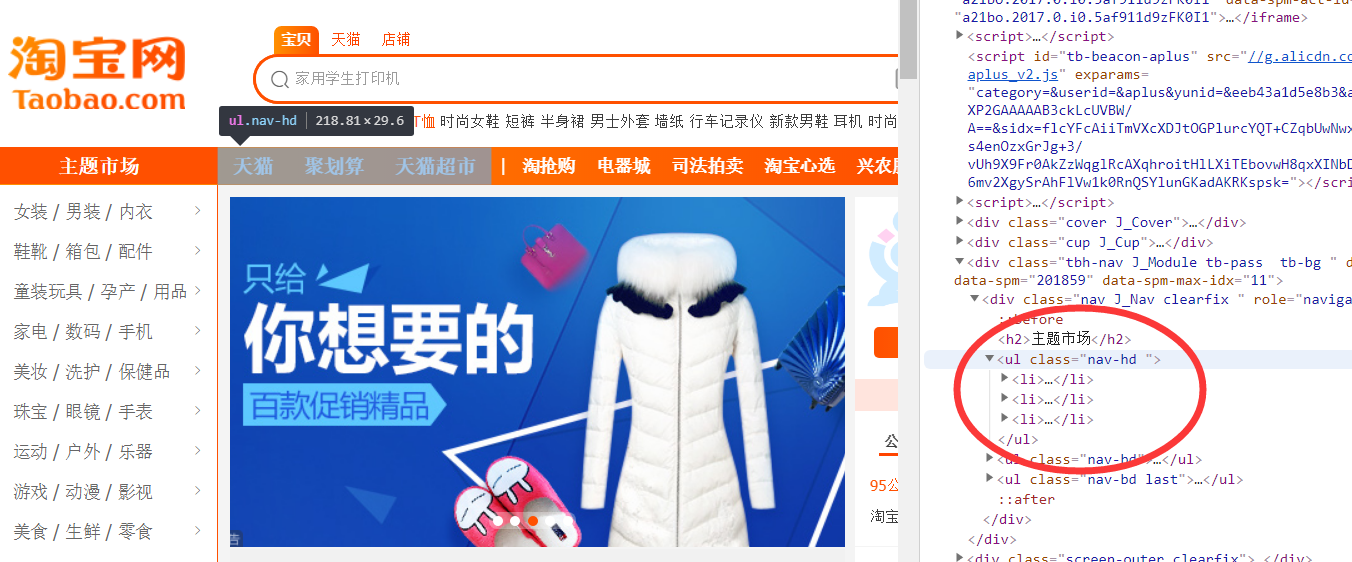
\includegraphics[scale=0.5]{img/C3/3-2/2.png}
    \caption{淘宝导航栏}
\end{figure}

\begin{lstlisting}[style=htmlcssjs, title=淘宝导航栏]
<!DOCTYPE html>
<html lang="en">
<head>
    <meta charset="UTF-8">
    <title>淘宝</title>
    <style type="text/css">
        ul {
            list-style: none;   /* 无序列表前面不带点 */
        }

        li {
            float: left;
            margin: 20px;
            padding: 5px;
            color: #000;
        }

        li:hover {
            background-color: #f40;     /* 淘宝红 */
            color: #fff;
            border-radius: 15px;
            cursor: pointer;
        }
    </style>
</head>
<body>
    <ul>
        <li>天猫</li>
        <li>聚划算</li>
        <li>天猫超市</li>
    </ul>
</body>
</html>
\end{lstlisting}

\newpage

\section{不发一张自拍吗?——img标签}

\subsection{img标签}

在网页的制作中为使网页炫丽美观,肯定是缺少不了图片,\lstinline|<img>|用于插入图片。 \\

\begin{lstlisting}[style=htmlcssjs]
<img src="图片地址" alt="下载失败时的替换文本" title="提示文本">
\end{lstlisting}

\begin{itemize}
    \item src属性用于标识图像的资源地址,资源地址可以来源于网上的URL,也可以来源于本地。

    \item alt属性指定图像的描述性文本,当图像下载不成功时,可看到该属性指定的文本。

    \item title属性提供当鼠标停留在图片时显示的文本。
\end{itemize}

\begin{lstlisting}[style=htmlcssjs, title=img标签, breaklines=true, breakatwhitespace=false]
<!DOCTYPE html>
<html lang="en">
<head>
    <meta charset="UTF-8">
    <title>img标签</title>
</head>
<body>
    <img src="https://ss0.bdstatic.com/70cFuHSh_Q1YnxGkpoWK1HF6hhy/it/u=3014023147,616635741&fm=26&gp=0.jpg" alt="皮卡丘.jpg" title="皮卡丘">
</body>
</html>
\end{lstlisting}

\newpage

\section{百度一下,你就知道——a标签}

\subsection{a标签}

使用\lstinline|<a>|可实现超链接,它在网页制作中可以说是无处不在,只要有链接的地方,就会有这个标签。 \\

\begin{lstlisting}[style=htmlcssjs]
<a href="目标网址" title="鼠标停留显示的文本">链接显示的文本</a>
\end{lstlisting}

\lstinline|<a>|中title属性提供的功能是当鼠标停留在链接文字时显示这个属性的文本内容,这个属性在实际网页开发中作用很大,主要方便搜索引擎了解链接地址的内容(语义化更友好)。

\begin{lstlisting}[style=htmlcssjs, title=a标签]
<!DOCTYPE html>
<html lang="en">
<head>
    <meta charset="UTF-8">
    <title>a标签</title>
</head>
<body>
    <a href="http://www.baidu.com" title="点击跳转百度">
        百度一下,你就知道
    </a>
</body>
</html>
\end{lstlisting}

只要为文本加入\lstinline|<a>|后,文字的颜色就会自动变为蓝色,被点击过的文本颜色会变为紫色,通过CSS样式可以对文字的颜色进行修改。 \\

\lstinline|<a>|中还有一个target属性,默认值为\_self,表示在同页面中打开被链接的文档。如果需要在新窗口打开被链接的文档,需要将target属性的值设置为\_blank。

\subsection{锚点(Anchor)}

\lstinline|<a>|最初的功能是记录锚点(记录位置),通过\lstinline|<a>|回到那个位置去。

\begin{lstlisting}[style=htmlcssjs, title=锚点, breaklines=true, breakatwhitespace=false]
<!DOCTYPE html>
<html lang="en">
<head>
    <meta charset="UTF-8">
    <title>锚点</title>
</head>
<body>
    <div id="div1" style="width: 100px; height: 100px; background-color: red;"></div>
    <div id="div2" style="width: 100px; height: 100px; background-color: blue;"></div>
    <br><br><br><br><br><br><br><br><br><br><br><br><br><br><br><br><br><br><br><br><br><br><br><br><br><br><br><br><br><br><br><br><br><br><br><br><br><br><br><br><br><br><br><br><br><br><br><br><br><br>
    <a href="#div1">跳转到div1</a>
    <a href="#div2">跳转到div2</a>
</body>
</html>
\end{lstlisting}

\lstinline|<a>|作为锚点的应用场景也很多,比如目录跳转。

\begin{figure}[H]
    \centering
    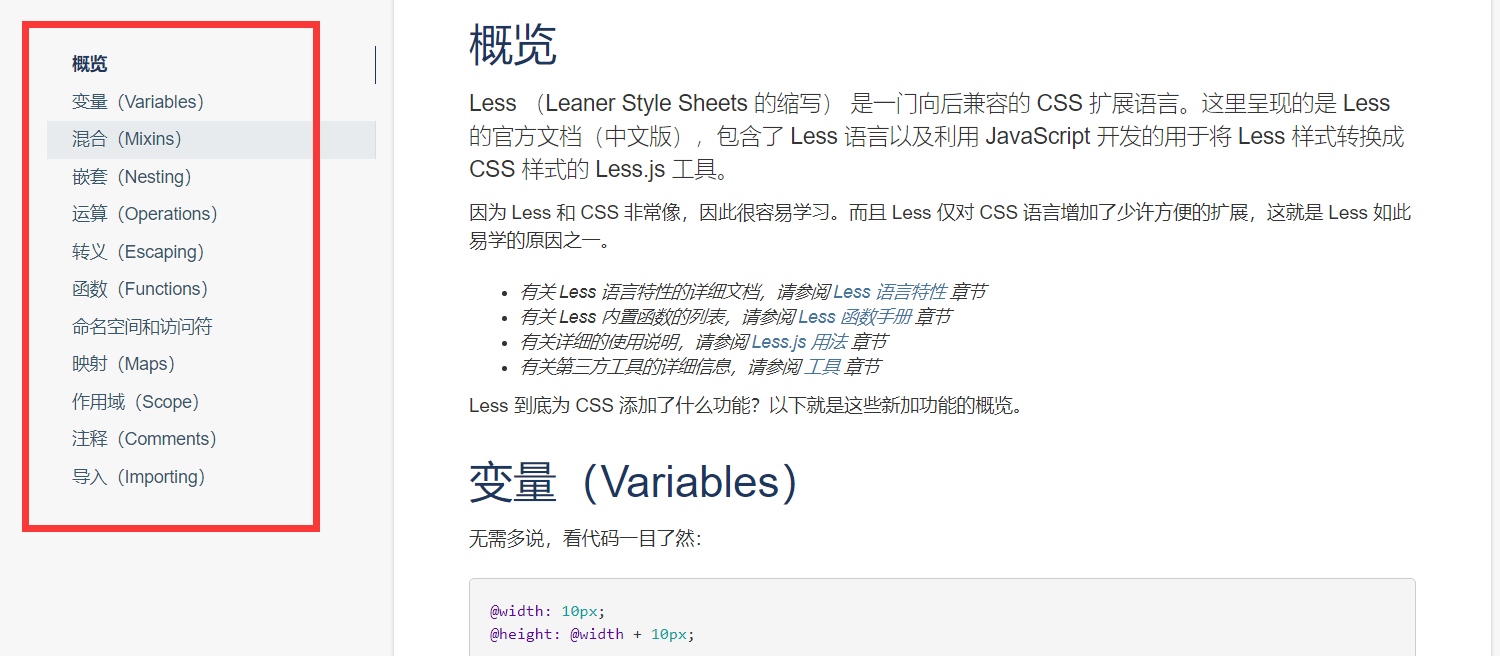
\includegraphics[scale=0.45]{img/C3/3-4/1.png}
    \caption{目录跳转}
\end{figure}

\subsection{协议限定符}

\lstinline|<a>|还能作为协议限定符,在点击链接时会强制执行JavaScript代码。

\begin{lstlisting}[style=htmlcssjs, title=协议限定符]
<!DOCTYPE html>
<html lang="en">
<head>
    <meta charset="UTF-8">
    <title>访问限定符</title>
</head>
<body>
    <a href="JavaScript: while(1) { alert('嘿嘿'); }">点我</a>
</body>
</html>
\end{lstlisting}

\newpage
\chapter{表格、表单}

\section{table标签}

\subsection{table标签}

有时候需要在网页中添加一些表格数据,如企业员工通讯录等。

\begin{figure}[H]
    \centering
    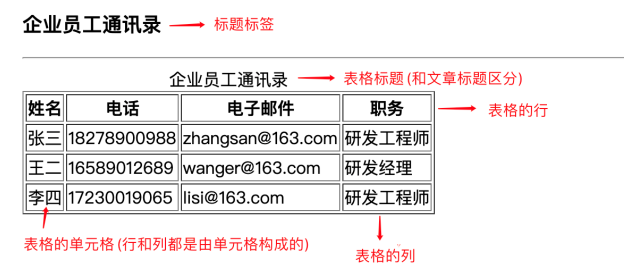
\includegraphics[scale=0.9]{img/C4/4-1/1.png}
    \caption{企业员工通讯录}
\end{figure}

创建表格主要包含5个元素:

\begin{enumerate}
    \item \lstinline|<caption>|:定义表格的标题。

    \item \lstinline|<table>|:整个表格以\lstinline|<table>|开始、\lstinline|</table>|结束,\lstinline|<table>|在没有添加border属性之前,在浏览器中显示是没有表格线的。

    \item \lstinline|<tr>|:表格的一行,有几对\lstinline|<tr>|表格就有几行,\lstinline|<tr>|里只能放\lstinline|<th>|或者\lstinline|<td>|。

    \item \lstinline|<th>|:表格头部的一个单元格,会加粗居中显示。

    \item \lstinline|<td>|:表格的一个单元格,有几对\lstinline|<td>|一行中就有几列。
\end{enumerate}

\begin{lstlisting}[style=htmlcssjs, title=企业员工通讯录]
<!DOCTYPE html>
<html lang="en">
<head>
    <meta charset="UTF-8">
    <title>企业员工通讯录</title>
</head>
<body>
    <h3>企业员工通讯录</h3>
    <hr/>

    <!-- 表格标签 border属性代表给表格加上边框 -->
    <table border="1">
        <!-- 表格标题 -->
        <caption>企业员工通讯录</caption>
        <!-- tr代表一行 -->
        <tr>
            <!-- th代表表格头部的一个单元格 -->
            <th>姓名</th>
            <th>电话</th>
            <th>电子邮件</th>
            <th>职务</th>
        </tr>
        <tr>
            <!-- td代表一个单元格 -->
            <td>张三</td>
            <td>18278900988</td>
            <td>zhangsan@163.com</td>
            <td>研发工程师</td>
        </tr>
        <tr>
            <td>王二</td>
            <td>16589012689</td>
            <td>wanger@163.com</td>
            <td>研发经理</td>
        </tr>
        <tr>
            <td>李四</td>
            <td>17230019065</td>
            <td>lisi@163.com</td>
            <td>研发工程师</td>
        </tr>
    </table>
</body>
</html>
\end{lstlisting}

\newpage

\section{与用户交互——form标签}

\subsection{form标签}

使用HTML表单(form)可以实现网站与用户的交互,表单可以把浏览者输入的数据传送到服务器端,这样服务器端程序就可以处理表单传过来的数据。 \\

\begin{lstlisting}[style=htmlcssjs]
<form method="传送方式" action="服务器文件">表单内容</form>
\end{lstlisting}

\lstinline|<form>|是成对出现的,以\lstinline|<form>|开始、\lstinline|</form>|结束。method属性表示数据传送的方式,包括get和post两种方式,get和post的区别属于后端程序员需要考虑的问题,完全取决于后端人员要求什么方式进行传输。action属性表示浏览者输入的数据被传送到的地方,比如一个PHP页面。 \\

所有的表单控件(文本框、文本域、按钮、单选框、复选框等)都必须放在\lstinline|<form>|之间,否则用户输入的信息无法提交到服务器上。

\newpage

\section{先来填用户名和密码——文本、密码输入框}

\subsection{文本、密码输入框}

当用户需要在表单中输入字母、数字等内容时,就需要使用到文本输入框,文本框也可转化为密码输入框。 \\

\begin{lstlisting}[style=htmlcssjs]
<form>
    <input type="text/password" name="名称" value="文本" />
</form>
<form>
    <input type="text/password" name="名称" value="文本" />
</form>
\end{lstlisting}

\begin{itemize}
    \item \lstinline|type="text"|:输入框为文本输入框
    \item \lstinline|type="password"|:输入框为密码输入框
    \item name:为文本框命名,以备后台程序使用
    \item value:为文本输入框设置默认值,一般起提示作用
\end{itemize}

\subsection{给点提示呗——placeholder属性}

有时候需要提示用户输入框需要输入的内容,这时候就需要使用\lstinline|<input>|中的占位符placeholder属性。

\begin{figure}[H]
    \centering
    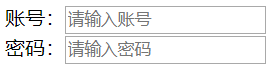
\includegraphics[]{img/C4/4-3/1.png}
    \caption{placeholder提示文本}
\end{figure}

placeholder属性的值可以根据情况合理填写,当输入框输入内容时,占位符内容消失,当输入框无内容时,占位符内容显示。注意,占位符内容不是输入框真正的内容。

\subsection{重置按钮}

当用户需要重置表单信息到初始状态时,比如输入“账号”或“密码”有误,就可以使用重置按钮使输入框恢复到初始状态。通过设置\lstinline|<input>|中type属性为reset即可实现重置按钮。

\subsection{提交按钮}

当用户需要提交表单信息到服务器时,需要用到提交按钮。通过设置\lstinline|<input>|中type属性为submit即可实现提交按钮。表单信息会被发送给后端,在数据库对比账户和密码信息。

\begin{lstlisting}[style=htmlcssjs, title=登录功能]
<!DOCTYPE html>
<html lang="en">
<head>
    <meta charset="UTF-8">
    <title>登录</title>
</head>
<body>
    <form action="get/post">
        账号:<input type="text" placeholder="请输入账号" name="username">
        <br/>
        密码:<input type="password" placeholder="请输入密码" name="password">
        <br/>
        <input type="submit">
        <input type="reset">
    </form>
</body>
</html>
\end{lstlisting}

\newpage

\section{数字、网址、邮箱输入框}

\subsection{数字输入框}

将\lstinline|<input>|的type属性设置为number,则表示该输入框的类型为数字。数字框只能输入数字,输入其它字符无效。数字框最右侧会有一个加减符号,可以调整输入数字的大小,不同浏览器表现不一致。

\subsection{网址输入框}

将\lstinline|<input>|的type属性设置为url,则表示输入类型为网址。网址输入框必须以http://或https://开头,且后面必须有内容,否则表单提交的时候会报错误提示。

\subsection{邮箱输入框}

将\lstinline|<input>|的type属性设置为email,则表示该输入框的类型为邮箱。邮箱输入框的值必须包含`@`,并且之后必须有内容,否则会报错误提示。

\begin{lstlisting}[style=htmlcssjs, title=个人信息]
<!DOCTYPE html>
<html lang="en">
<head>
    <meta charset="UTF-8">
    <title>个人信息</title>
</head>
<body>
    <form action="get/post">
        姓名:<input type="text" name="name"><br/>
        年龄:<input type="number" name="age"><br/>
        主页:<input type="url" name="webpage"><br/>
        邮箱:<input type="email" name="email"><br/>
        <input type="submit">
        <input type="reset">
    </form>
</body>
</html>
\end{lstlisting}

\newpage

\section{文本域}

\subsection{文本域}

当用户需要在表单中输入大段文字时,就需要用到文本输入域。\lstinline|<textarea>|中也可以设置placeholder属性来显示提示信息。 \\

\begin{lstlisting}[style=htmlcssjs]
<textarea rows="行数" cols="列数">文本</textarea>
\end{lstlisting}

\begin{itemize}
    \item rows:多行输入域的行数,可以用CSS样式的height代替
    \item cols:多行输入域的列数,可以用CSS样式的width代替
\end{itemize}

\begin{lstlisting}[style=htmlcssjs, title=文本域]
<!DOCTYPE html>
<html lang="en">
<head>
    <meta charset="UTF-8">
    <title>文本域</title>
</head>
<body>
    <form action="get/post">
        <textarea cols="30" rows="10" placeholder="请输入..."></textarea>
    </form>
</body>
</html>
\end{lstlisting}

\newpage

\section{label标签}

\subsection{label标签}

\lstinline|<label>|不会向用户呈现任何特殊特效,它的作用是为鼠标用户改进了可用性。如果在\lstinline|<label>|内点击文本,就会触发此控件。也就是说,当用户单击选中该\lstinline|<label>|时,浏览器就会自动将焦点转到和标签相关的表单控件上。

\begin{lstlisting}[style=htmlcssjs]
<label for="控件id名称">
\end{lstlisting}

注意,\lstinline|<label>|的for属性的值必须要与相关空间的id属性值相同。

\begin{lstlisting}[style=htmlcssjs, title=label标签]
<!DOCTYPE html>
<html lang="en">
<head>
    <meta charset="UTF-8">
    <title>label标签</title>
</head>
<body>
    <form action="get/post">
        <label for="username">用户名:</label>
        <input type="text" id="username">
    </form>
</body>
</html>
\end{lstlisting}

\newpage

\section{单选框、复选框}

\subsection{单选框、复选框}

在使用表单设计调查表时,为了减少用户的操作,使用选择框是一个好主意。HTML中有两种选择框,即单选框和复选框,两者的区别是单选框中的选项用户只能选择一项,而复选框中用户可以任意选择多项,甚至全选。 \\

\begin{lstlisting}[style=htmlcssjs]
<input type="radio/checkbox" name="名称" value="值" checked="checked">
\end{lstlisting}

\begin{itemize}
    \item \lstinline|type="radio"|:单选框
    \item \lstinline|type="checkbox"|:复选框
    \item name:为控件命名,具有相同名称的选择框属于同一组
    \item checked:设置默认选中的值
\end{itemize}

在网页开发中,往往需要优化用户体验。一个好的产品有3个特点:解决刚需的问题、用户体验、用户黏性(产品定位)。用户体验就是养成用户的懒习惯,减少用户操作,能不让用户操作就不让用户操作,节省用户时间,用户不动手就会觉得方便。例如一个选择性别的单选框,概率上看,假设有100个人,50男50女,使用默认选项,可以节省一半人的操作。

\begin{lstlisting}[style=htmlcssjs, title=单选框/复选框]
<!DOCTYPE html>
<html lang="en">
<head>
    <meta charset="UTF-8">
    <title>单选框/复选框</title>
</head>
<body>
    <form action="get/post">
        1. 您是否喜欢运动?
        <input type="radio" name="sport" checked="checked">是
        <input type="radio" name="sport">否
        2. 您喜欢的运动是?
        <input type="checkbox" name="sport_item">跑步
        <input type="checkbox" name="sport_item">篮球
        <input type="checkbox" name="sport_item">羽毛球
    </form>
</body>
</html>
\end{lstlisting}

\newpage

\section{下拉列表}

\subsection{下拉列表}

下拉列表在网页中也常会用到,它可以有效的节省网页空间。下拉列表既可以单选也可以多选。 \\

\begin{lstlisting}[style=htmlcssjs]
<select>
    <option value="值">选项</option>
    <option value="值">选项</option>
</select>
\end{lstlisting}

\begin{itemize}
    \item value:向服务器提交的值,而双标签中间的内容才是显示的值
    \item selected:设置\lstinline|selected="selected"|表示该选项被默认选中
\end{itemize}

\begin{lstlisting}[style=htmlcssjs, title=下拉列表]
<!DOCTYPE html>
<html lang="en">
<head>
    <meta charset="UTF-8">
    <title>下拉列表</title>
</head>
<body>
    <form action="get/post">
        <select>
            <option value="male" selected="selected">男</option>
            <option value="female">女</option>
        </select>
    </form>
</body>
</html>
\end{lstlisting}

\newpage
\part{CSS}

\newpage

\chapter{CSS简介}

\section{给HTML打扮——CSS样式}

\subsection{层叠样式表(CSS, Cascading Style Sheets)}

CSS主要用于定义HTML内容在浏览器内的显示样式,如文字大小、颜色、字体加粗等。使用CSS样式的一个好处是通过定义某个样式,可以让不同网页位置的问题有着统一的字体、字号或颜色等。CSS样式由选择器和声明组成,而声明又由属性和值组成。 \\

\begin{lstlisting}[style=htmlcssjs]
selector {
    attribute: value;
}
\end{lstlisting}

选择器也称选择符,用于指明网页中要应用样式规则的元素。声明的内容写在大括号【{}】内,属性和值之前用冒号【:】分隔。当有多条声明时,中间可以用分号【;】分隔。 最后一条声明可以没有分号,但是为了后续修改方便,一般也加上分号。为了使样式更加容易阅读,可以将每条声明单独成行。

\begin{lstlisting}[style=htmlcssjs, title=修改字体大小和颜色]
<!DOCTYPE html>
<html lang="en">
<head>
    <meta charset="UTF-8">
    <title>修改字体大小和颜色</title>
    <style type="text/css">
        p {
            font-size: 20px;
            color: red;
        }
    </style>
</head>
<body>
    <p>修改字体大小和颜色</p>
</body>
</html>
\end{lstlisting}

\newpage

\section{既然那么好,那就引入CSS吧——内联式CSS}

\subsection{内联式CSS}

内联式CSS样式,也称行间样式,就是把CSS代码直接写在现有的HTML标签中。注意CSS样式必须写在元素的开始标签里,不能在结束标签里。 \\


\chapter{选择器}

\section{选一个标签——标签选择器}

\subsection{标签选择器}

标签选择器其实就是HTML代码中的标签。 \\

\begin{lstlisting}[style=htmlcssjs]
tag_selector {
    attribute: value;
}
\end{lstlisting}

\begin{lstlisting}[style=htmlcssjs, title=标签选择器]
<!DOCTYPE html>
<html lang="en">
<head>
    <meta charset="UTF-8">
    <title>标签选择器</title>
    <style type="text/css">
        h2 {
            color: green;
            font-size: 30px;
        }
    </style>
</head>
<body>
    <h2>CSS特点</h2>
    <p>CSS为HTML标记语言提供了一种样式描述。</p>
</body>
</html>
\end{lstlisting}

\newpage

\section{再选一个类——类选择器}

\subsection{类选择器}

类选择器在CSS样式中是最常用的。类选择器使用【.】开头,后加类选择器的名称,CSS样式代码会被作用到属于该类的HTML标签中。在标签中使用class属性为标签设置一个类。 \\

类选择器与标签是多对多的关系,即类选择器名称可以多个标签共用,一个元素可以用多个class,一个class值可以对应多个元素。多个class值之间使用空格分隔。

\begin{lstlisting}[style=htmlcssjs, title=类选择器]
<!DOCTYPE html>
<html lang="en">
<head>
    <meta charset="UTF-8">
    <title>类选择器</title>
    <style type="text/css">
        .title {
            color: green;
        }
    </style>
</head>
<body>
    <h3 class="title">丰富的样式定义</h3>
    <p>CSS提供了丰富的文档样式外观。</p>
    <h3 class="title">易于使用和修改</h3>
    <p>CSS样式表可以将所有的样式声明统一存放,进行统一管理。</p>
</body>
</html>
\end{lstlisting}

\newpage

\section{取个唯一表示——ID选择器}

\subsection{ID选择器}

使用ID选择器,必须给标签添加上id属性,即为标签设置id属性。ID选择器名称的前面使用【\#】。 \\

ID选择器与标签是一对一的关系,即一个元素只能有一个id值,一个id值只能对应一个元素。id是全局唯一的,就像身份证号码一样。

\begin{lstlisting}[style=htmlcssjs, title=ID选择器]
<!DOCTYPE html>
<html lang="en">
<head>
    <meta charset="UTF-8">
    <title>ID选择器</title>
    <style type="text/css">
        div {
            width: 100px;
            height: 100px;
        }

        #square1 {
            background-color: red;
        }
        #square2 {
            background-color: blue;
        }
    </style>
</head>
<body>
    <div id="square1"></div>
    <div id="square2"></div>
</body>
</html>
\end{lstlisting}

\newpage

\section{捡了个儿子——子选择器}

\subsection{子选择器}

子选择器【>】,用于选择指定标签元素的第一代子元素。

\begin{lstlisting}[style=htmlcssjs, title=子选择器]
<!DOCTYPE html>
<html lang="en">
<head>
    <meta charset="UTF-8">
    <title>子选择器</title>
    <style type="text/css">
        .food > li {
            border: 1px solid red;
        }
    </style>
</head>
<body>
    <h2>食物</h2>
    <ul class="food">
        <li>水果
            <ul>
                <li>苹果</li>
                <li>香蕉</li>
            </ul>
        </li>
        <li>蔬菜
            <ul>
                <li>白菜</li>
                <li>油菜</li>
            </ul>
        </li>
    </ul>
</body>
</html>
\end{lstlisting}

\newpage

\section{这么快就当爷爷了——后代选择器}

\subsection{后代选择器}

后代选择器,也称包含选择器,用于选择指定标签元素的后辈元素。 \\

\begin{lstlisting}[style=htmlcssjs]
ancestor_selector descendant_selector {
    attribute: value;
}
\end{lstlisting}

后代选择器与子选择器的区别在于,子选择器仅是指它的直接后代,而后代选择器是作用于所有子后代元素。

\begin{lstlisting}[style=htmlcssjs, title=后代选择器]
<!DOCTYPE html>
<html lang="en">
<head>
    <meta charset="UTF-8">
    <title>后代选择器</title>
    <style type="text/css">
        .food li {
            border: 1px solid red;
        }
    </style>
</head>
<body>
    <h2>食物</h2>
    <ul class="food">
        <li>
            水果
            <ul>
                <li>苹果</li>
                <li>香蕉</li>
                <li>橘子</li>
            </ul>
        </li>
        <li>
            蔬菜
            <ul>
                <li>白菜</li>
                <li>油菜</li>
                <li>卷心菜</li>
            </ul>
        </li>
    </ul>
</body>
</html>
\end{lstlisting}

\newpage

\section{我全都要——通配符选择器}

\subsection{通配符选择器}


\chapter{字体、文本样式}

\section{字体样式}

\subsection{字体样式}

使用CSS样式可以为网页中的文字设置字体。注意不要设置不常用的字体,因为如果用户本地电脑上没有安装该字体,就会显示浏览器默认的字体。 \\

浏览器默认的字号为16px,使用font-size可以修改字号大小。 \\

为文字设置粗体是有单独的CSS样式来实现的,再也不用为了实现粗体样式而使用\lstinline|<h1>|-\lstinline|<h6>|或\lstinline|<strong>|了。 \\

font-weight的默认值为normal,通过设置属性值为lighter、bold、bolder或100-900之间的整百数值改变文字的粗细。注意,字体能否被bolder或lighter更改取决于字体包是否存在该样式。 \\

font-style可以设置字体样式,并且有3种设置方式:

\begin{enumerate}
    \item 正常字体为normal,也是font-style的默认值
    \item italic为字体设置为斜体,用于字体本身就有倾斜的样式
    \item oblique强制将字体倾斜
\end{enumerate}

\begin{lstlisting}[style=htmlcssjs, title=字体样式]
<!DOCTYPE html>
<html lang="en">
<head>
    <meta charset="UTF-8">
    <title>字体样式</title>
    <style type="text/css">
        p {
            font-family: "arial";
            font-size: 20px;
            font-weight: bold;
            font-style: italic;
        }   
    </style>
</head>
<body>
    <p>Cascading Style Sheets (CSS) is a style sheet language used for describing the presentation of a document written in a markup language such as HTML.</p>
</body>
</html>
\end{lstlisting}

\newpage


\chapter{盒子模型与布局模型}

\section{元素分类}

\subsection{我要独占一行——块级元素}

在HTML中\lstinline|<div>|、\lstinline|<p>|、\lstinline|<h1>|、\lstinline|<form>|、\lstinline|<ul>|、\lstinline|<li>|等都是块级元素。每个块级元素都从新的一行开始,并且其后的元素也另起一行。块级元素的高度、宽度、行高遗迹顶和底边距都可以设置,宽度在不设定的情况下,是它本身父容器的100\%(和父元素的宽度一致)。

\begin{lstlisting}[style=htmlcssjs, title=块级元素]
<!DOCTYPE html>
<html lang="en">
<head>
    <meta charset="UTF-8">
    <title>块级元素</title>
</head>
<body>
    <div>这是一个div标签</div>
    <p>这是一个p标签</p>
    <h1>这是一个h1标签</h1>
</body>
</html>
\end{lstlisting}

通过设置\lstinline|display: block|可以将元素显示为块级元素。

\subsection{我要和你站一起——内联元素}

在HTML中,\lstinline|<span>|、\lstinline|<a>|、\lstinline|<label>|、\lstinline|<strong>|、\lstinline|<em>|等都是内联元素(行内元素)。内联元素和其它元素都在一行上,元素的高度、宽度及顶部和底部编剧不可设置,元素的宽度就是它包含的文字或图片的宽度,不可改变。 \\

块级元素也可以设置\lstinline|display: inline|将元素设置为内联元素。

\begin{lstlisting}[style=htmlcssjs, title=内联元素与块级元素转换]
<!DOCTYPE html>
<html lang="en">
<head>
    <meta charset="UTF-8">
    <title>内联元素与块级元素转换</title>
    <style type="text/css">
        a {
            display: block;
        }

        div {
            display: inline;
        }
    </style>
</head>
<body>
    <a>我要变成块级元素</a>
    <a>我也要变成块级元素</a>

    <div>我要变成内联元素</div>
    <div>我也要变成内联元素</div>
</body>
</html>
\end{lstlisting}

\subsection{我还要占个大位置——内联块状元素}

内联块状元素就是同时具备内联元素和块级元素的特点。内联块状元素的特点是和其它元素都在一行上,但元素的高度、宽度、行高以及顶和底边距都可以设置。 \\

通过设置\lstinline|display: inline-block|就可以将元素设置为内联块状元素。如\lstinline|<img>|、\lstinline|<input>|就是这种内联块状标签。

\newpage

\section{盒子模型}

\subsection{盒子模型}

盒子模型包含4个部分:

\begin{enumerate}
    \item 外边距(margin)
    \item 外边框(border)
    \item 内边距(padding)
    \item 内容(content)
\end{enumerate}

\begin{figure}[H]
    \centering
    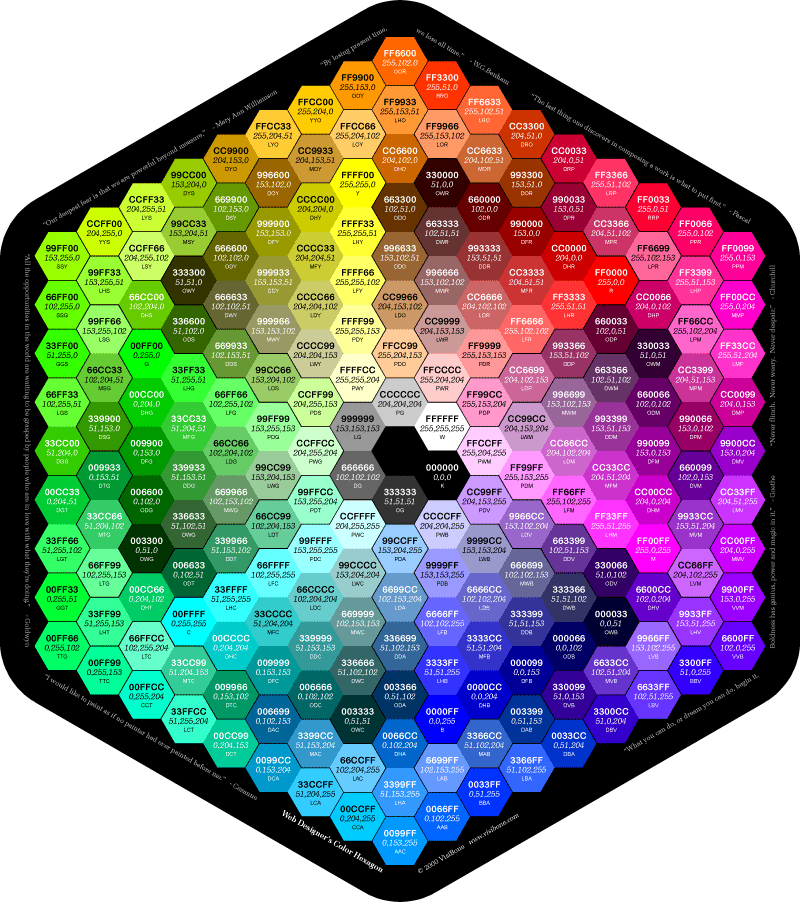
\includegraphics[scale=0.7]{img/C8/8-2/1.png}
\end{figure}

盒模型的宽度和高度和平常所说的物体的宽度和高度的理解是不一样的,CSS内定义的宽和高,指的是盒模型中内容的宽和高。 \\

元素实际的宽度(盒子的宽度) = 左外边距 + 左边框 + 左内边距 + 内容宽度 + 右内边距 + 右边框 + 右外边距 \\

\begin{figure}[H]
    \centering
    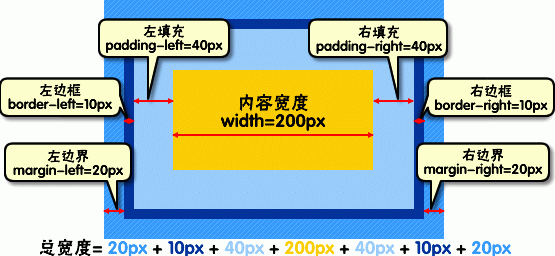
\includegraphics[]{img/C8/8-2/2.png}
\end{figure}

\subsection{外边框(Border)}

盒子模型的外边框可以设置粗细、样式和颜色:

\begin{enumerate}
    \item border-width:设置边框的宽度,常用单位为像素(px)
    \item border-style:边框样式包括实线solid、虚线dashed、点线dotted
    \item border-color:设置边框颜色
\end{enumerate}

当三个属性都需要被设置时,也可以使用border属性简写。例如设置一个粗细为1px实心的黑色边框: \\

\begin{lstlisting}[style=htmlcssjs]
border: 1px solid black;
\end{lstlisting}

CSS中也允许只为一个方向的边框设置属性,使用border-top、border-bottom、border-left、border-right可以单独设置上、下、左、右四条边框。 \\

元素边框的圆角效果可以使用border-radius属性来设置。设置圆角的值的顺序为左上、右上、右下、左下。如果border-radius属性只给出一个值表示四个圆角都被设置成该值。如果只给出两个值表示左上角和右下角设置为第一个值,右上角和左下角设置为第二个值。当给一个正方形的圆角效果值设置为其宽度一半时,显示效果为圆形。

\begin{lstlisting}[style=htmlcssjs, title=圆形]
<!DOCTYPE html>
<html lang="en">
<head>
    <meta charset="UTF-8">
    <title>圆形</title>
    <style type="text/css">
        div {
            width: 100px;
            height: 100px;
            background-color: red;
            border-radius: 50%;
        }
    </style>
</head>
<body>
    <div></div>
</body>
</html>
\end{lstlisting}

通过单独设置每条边的属性,可以在正方形内展现不同的颜色。

\begin{figure}[H]
    \centering
    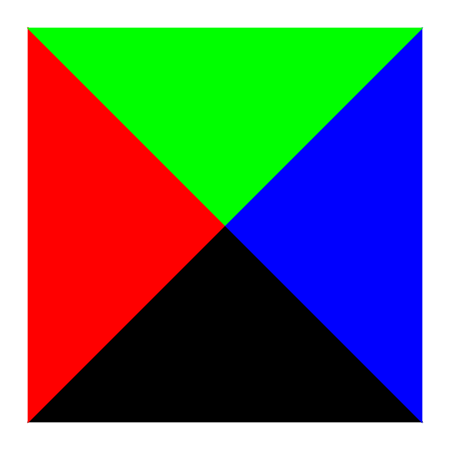
\begin{tikzpicture}
        \filldraw[draw=black, fill=black] (0,0) -- (5,0) -- (2.5,2.5) -- cycle;
        \filldraw[draw=red, fill=red] (0,0) -- (2.5,2.5) -- (0,5) -- cycle;
        \filldraw[draw=blue, fill=blue] (5,0) -- (2.5,2.5) -- (5,5) -- cycle;
        \filldraw[draw=green, fill=green] (2.5,2.5) -- (0,5) -- (5,5) -- cycle;
    \end{tikzpicture}
\end{figure}

\begin{lstlisting}[style=htmlcssjs, title=四色正方形]
<!DOCTYPE html>
<html lang="en">
<head>
    <meta charset="UTF-8">
    <title>四色正方形</title>
    <style type="text/css">
        div {
            width: 0;
            height: 0;
            border: 100px solid black;
            border-left-color: red;
            border-top-color: green;
            border-right-color: blue;
        }
    </style>
</head>
<body>
    <div></div>
</body>
</html>
\end{lstlisting}

通过设置透明色(transparent),可以绘制出三角形。

\begin{figure}[H]
    \centering
    
\begin{tikzpicture}
        \filldraw[draw=black, fill=black] (0,0) -- (5,0) -- (2.5,2.5) -- cycle;
        \filldraw[draw=black, fill=black] (0,0) -- (2.5,2.5) -- (0,5) -- cycle;
    \end{tikzpicture}
\end{figure}

\begin{lstlisting}[style=htmlcssjs, title=三角形]
<!DOCTYPE html>
<html lang="en">
<head>
    <meta charset="UTF-8">
    <title>三角形</title>
    <style type="text/css">
        div {
            width: 0;
            height: 0;
            border: 100px solid black;
            border-left-color: black;
            border-top-color: transparent;
            border-right-color: transparent;
        }
    </style>
</head>
<body>
    <div></div>
</body>
</html>
\end{lstlisting}

\subsection{内边距(Padding)}

元素内容与边框之间是可以设置距离的,称之为内边距或填充。内边距也可分为上、右、下、左(顺时针)。

\begin{figure}[H]
    \centering
    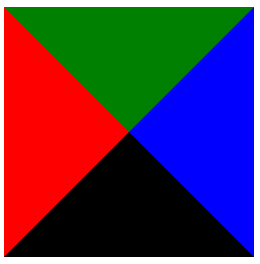
\includegraphics[scale=0.7]{img/C8/8-2/3.png}
\end{figure}

\subsection{外边距(Margin)}

元素与其他元素之间的距离可以使用外边距来设置,外边距也可分为上、右、下、左。

\begin{figure}[H]
    \centering
    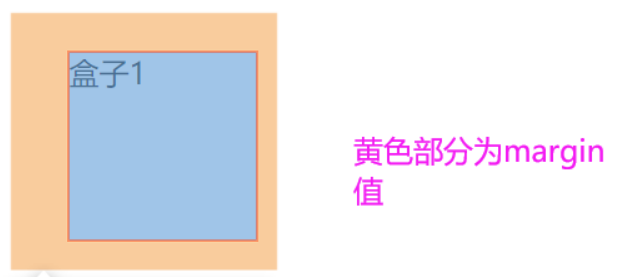
\includegraphics[scale=0.7]{img/C8/8-2/4.png}
\end{figure}

margin与padding的区别在于,padding在外边框里,margin在外边框外。

\newpage

\section{布局模型}

\subsection{布局模型}

布局模型建立在盒子模型的基础上,在网页中,元素有3种布局模型:

\begin{enumerate}
    \item 流动模型(flow)
    \item 浮动模型(float)
    \item 层模型(layer)
\end{enumerate}

\subsection{流动模型}

流动模型是默认的网页布局模式,也就是说网页在默认状态下的HTML网页元素都是根据流动模型来分布网页内容的。 \\

流动布局模型有2个典型的特征:

\begin{enumerate}
    \item 块级元素都会在所处的包含元素内自上而下按顺序垂直延伸分布,因为在默认状态下,块级元素的宽度都为100\%,即都会以行的形式占据位置。
          \begin{figure}[H]
              \centering
              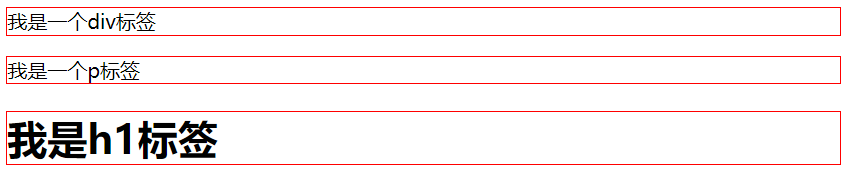
\includegraphics[scale=0.7]{img/C8/8-3/1.png}
          \end{figure}

    \item 内联元素都会在所处的包含元素内从左到右水平分布显示。
          \begin{figure}[H]
              \centering
              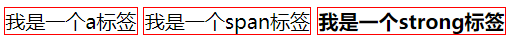
\includegraphics[]{img/C8/8-3/2.png}
          \end{figure}
\end{enumerate}

\subsection{浮动模型}

块级元素这么霸道都是独占一行,如果想让两个块级元素并排显示,可以设置元素浮动。任何元素在默认情况下是不能浮动的,但可以设置float属性定义为浮动,如\lstinline|<div>|、\lstinline|<p>|、\lstinline|<table>|、\lstinline|<img>|等元素都可以被定义为浮动。

\begin{lstlisting}[style=htmlcssjs, title=浮动模型]
<!DOCTYPE html>
<html lang="en">
<head>
    <meta charset="UTF-8">
    <title>浮动模型</title>
    <style type="text/css">
        div {
            width: 100px;
            height: 100px;
            border: 1px solid red;
        }

        #div1 {
            float: left;
        }

        #div2 {
            float: right;
        }
    </style>
</head>
<body>
    <div id="div1"></div>
    <div id="div2"></div>
</body>
</html>
\end{lstlisting}

\newpage

\section{定位}

\subsection{层模型}

层布局模型就像是图像软件PhotoShop中非常流行的图层编辑功能一样,每个图形能够精确定位操作(positioning)。由于有些元素是定点展示的,定位技术可以让元素在特定的位置出现。 \\

层模型有3种形式:

\begin{enumerate}
    \item 绝对定位(absolute)
    \item 相对定位(relative)
    \item 固定定位(fixed)
\end{enumerate}

\subsection{万事无绝对——绝对定位}

如果想为元素设置层模型中的绝对定位,需要设置\lstinline|position: absolute|,这条语句的作用是将元素从文档流中拖出来,然后使用left、right、top、bottom属性相对于其最接近的一个具有定位属性的父包含块进行绝对定位。如果不存在这样的包含块,则相对于body元素,即相对于浏览器窗口。 \\

当一个元素成为绝对定位元素,它就脱离了原来的层面,原来的位置会空出,下面的元素都会上来。

\begin{lstlisting}[style=htmlcssjs, title=绝对定位]
<!DOCTYPE html>
<html lang="en">
<head>
    <meta charset="UTF-8">
    <title>绝对定位</title>
    <style type="text/css">
        div {
            width: 100px;
            height: 100px;
        }

        #div1 {
            background-color: red;
            position: absolute;
            top: 50px;      /* 距离窗口上边50px */
            left: 100px;    /* 距离窗口左边100px */
        }

        #div2 {
            background-color: blue;
        }
    </style>
</head>
<body>
    <div id="div1"></div>
    <div id="div2"></div>
</body>
</html>
\end{lstlisting}

\begin{figure}[H]
    \centering
    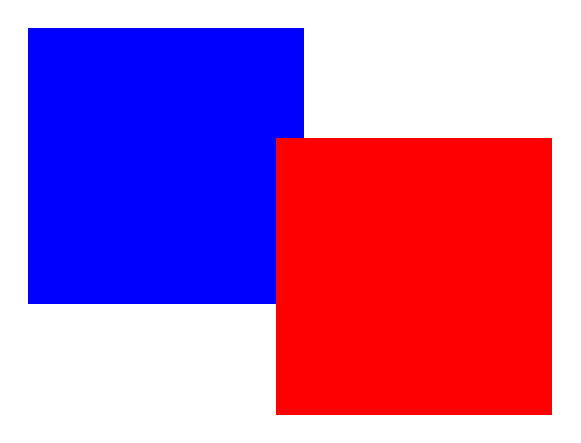
\begin{tikzpicture}[scale=0.7]
        \filldraw[draw=blue, fill=blue] (0,2) -- (0,7) -- (5,7) -- (5,2) -- cycle;
        \filldraw[draw=red, fill=red] (4.5,0) -- (9.5,0) -- (9.5,5) -- (4.5,5) -- cycle;
    \end{tikzpicture}
\end{figure}

\subsection{相对于自己的位置——相对定位}

如果想为元素设置层模型中的相对定位,需要设置\lstinline|position: relative|,它通过left、right、top、bottom属性确定元素在正常文档流中的偏移位置。相对定位完成的过程是首先按static (float)方式生成一个元素,然后相对于以前的位置移动,并且偏移前的位置保留不动,因此下面的元素无法上来。

\begin{lstlisting}[style=htmlcssjs, title=相对定位]
<!DOCTYPE html>
<html lang="en">
<head>
    <meta charset="UTF-8">
    <title>相对定位</title>
    <style type="text/css">
        div {
            width: 100px;
            height: 100px;
        }

        #div1 {
            background-color: red;
            position: relative;
            top: 50px;
            left: 100px;
        }

        #div2 {
            background-color: blue;
        }
    </style>
</head>
<body>
    <div id="div1"></div>
    <div id="div2"></div>
</body>
</html>
\end{lstlisting}

\begin{figure}[H]
    \centering
    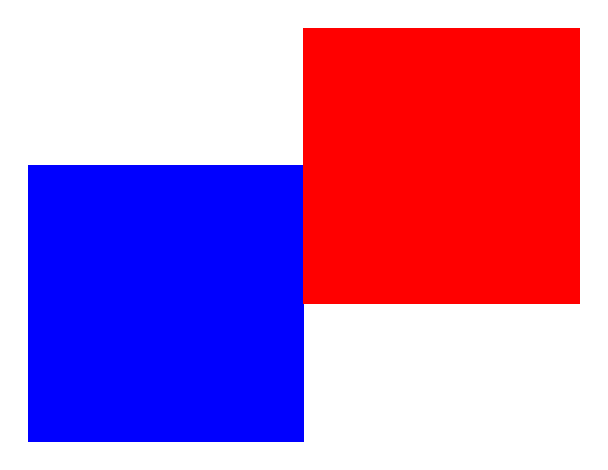
\begin{tikzpicture}[scale=0.7]
        \filldraw[draw=blue, fill=blue] (0,0) -- (0,5) -- (5,5) -- (5,0) -- cycle;
        \filldraw[draw=red, fill=red] (5,2.5) -- (5,7.5) -- (10,7.5) -- (10,2.5) -- cycle;
    \end{tikzpicture}
\end{figure}

使用\lstinline|position: absolute|可以实现元素相对于浏览器(body)设置定位,那可不可以相对于其它元素进行定位呢?当然可以,但是必须要满足以下的3点条件:

\begin{enumerate}
    \item 参照定位的元素必须是相对定位元素的前辈元素。
    \item 参照定位的元素必须加入\lstinline|position: relative|。
    \item 定位元素加入`position: absolute`后便可以使用top、bottom、left、right来进行偏移了。
\end{enumerate}

\begin{lstlisting}[style=htmlcssjs, title=相对父元素定位]
<!DOCTYPE html>
<html lang="en">
<head>
    <meta charset="UTF-8">
    <title>相对父元素定位</title>
    <style type="text/css">
        #div1 {
            width: 100px;
            height: 100px;
            background-color: red;
            position: relative;
        }

        #div2 {
            width: 100px;
            height: 20px;
            background-color: blue;
            position: absolute;
            top: 40px;
        }
    </style>
</head>
<body>
    <div id="div1">
        <div id="div2"></div>
    </div>
</body>
</html>
\end{lstlisting}

\begin{figure}[H]
    \centering
    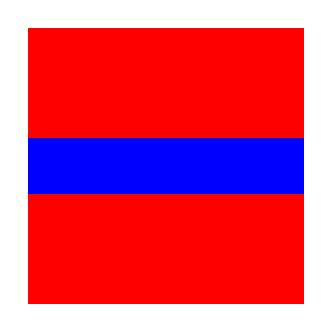
\begin{tikzpicture}[scale=0.7]
        \filldraw[draw=red, fill=red] (0,0) -- (0,5) -- (5,5) -- (5,0) -- cycle;
        \filldraw[draw=blue, fill=blue] (0,2) -- (0,3) -- (5,3) -- (5,2) -- cycle;
    \end{tikzpicture}
\end{figure}

\subsection{我就在那不动了——固定定位}

通过设置\lstinline|position: fixed|让一个元素固定在一个位置,它的相对移动的坐标是视图(屏幕内的网页窗口)本身。由于视图本身是固定的,它不会随着浏览器窗口的滚动条滚动而变化,除非在屏幕中移动浏览器窗口的屏幕位置,或改变浏览器窗口的显示大小。因此固定定位的元素会始终位于浏览器窗口内视图的某个位置,不会受文档流影响。

\begin{lstlisting}[style=htmlcssjs, title=固定定位, breaklines=true, breakatwhitespace=false]
<!DOCTYPE html>
<html lang="en">
<head>
    <meta charset="UTF-8">
    <title>固定定位</title>
    <style type="text/css">
        img {
            position: fixed;
            top: 15%;
            left: 20%;
        }
    </style>
</head>
<body>
    <img src="https://gimg2.baidu.com/image_search/src=http%3A%2F%2Fc-ssl.duitang.com%2Fuploads%2Fitem%2F201702%2F02%2F20170202151743_rvLWi.jpeg&refer=http%3A%2F%2Fc-ssl.duitang.com&app=2002&size=f9999,10000&q=a80&n=0&g=0n&fmt=jpeg?sec=1618588336&t=2612dc782456b9fdb8eeac0d0a215a85" alt="灰原哀.jpg" title="灰原哀">
    <br><br><br><br><br><br><br><br><br><br><br><br><br><br><br><br><br><br><br><br><br><br><br><br><br><br><br><br><br><br><br><br><br><br><br><br><br><br><br><br><br><br><br><br><br><br><br><br><br><br>
</body>
</html>
\end{lstlisting}

\mybox{奥运五环}

\begin{figure}[H]
    \centering
    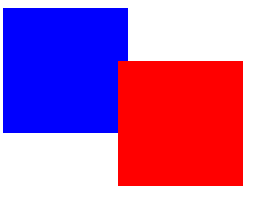
\includegraphics[scale=0.7]{img/C8/8-4/1.png}
\end{figure}

\begin{lstlisting}[style=htmlcssjs, title=olympic.html]
<!DOCTYPE html>
<html lang="en">
<head>
    <meta charset="UTF-8">
    <title>奥运五环</title>
    <link rel="stylesheet" type="text/css" href="olympic.css">
</head>
<body>
    <!-- 展示奥运五环的区域 -->
    <div class="stage">
        <div id="circle1"></div>
        <div id="circle2"></div>
        <div id="circle3"></div>
        <div id="circle4"></div>
        <div id="circle5"></div>
    </div>
</body>
</html>
\end{lstlisting}

\begin{lstlisting}[style=htmlcssjs, title=olympic.css]
* {
        margin: 0;
        padding: 0;
    }
    
    .stage {
        position: absolute;
        left: 50%;
        top: 50%;
        margin-left: -190px;
        margin-top: -93px;
        height: 185px;
        width: 380px;
    }
    
    #circle1,
    #circle2,
    #circle3,
    #circle4,
    #circle5 {
        position: absolute;
        width: 100px;
        height: 100px;
        border: 10px solid black;
        border-radius: 50%;
    }
    
    #circle1 {
        border-color: blue;
        left: 0;
        top: 0;
    }
    
    #circle2 {
        border-color: black;
        left: 130px;
        top: 0;
    }
    
    #circle3 {
        border-color: red;
        left: 260px;
        top: 0;
    }
    
    #circle4 {
        border-color: yellow;
        left: 65px;
        top: 70px;
    }
    
    #circle5 {
        border-color: green;
        left: 195px;
        top: 70px;
    }
\end{lstlisting}

\newpage

\end{document}